%
% chapter.tex
%
% (c) 2020 Prof Dr Andreas Müller
%
\chapter{Berechnung
\label{chapter:berechnung}}
\lhead{Berechnung}
\rhead{}
Die numerischen Datentypen eines digitalen Computers sind Approximationen
für die abstrakten Zahlensysteme $\mathbb{N}$, $\mathbb{Z}$, $\mathbb{Q}$
und $\mathbb{R}$.
\index{Zahlensystem}%
\index{R@$\mathbb R$}%
\index{N@$\mathbb N$}%
\index{Z@$\mathbb Z$}%
\index{Q@$\mathbb Q$}%
Man kann sie daher verwenden, die in der Analysis und der linearen Algebra
definierten Konzepte wie Grenzwerte, Integrale oder inverse Matrizen zu
berechnen.
\index{lineare!Algebra}
Da sie jedoch nur Annäherungen sind, werden die gewohnten Rechenregeln 
nicht immer gültig sein.
\index{Rechenregeln}%
In $\mathbb{R}$ kann die Addition dreier Zahlen zum Beispiel in beliebiger
Reihenfolge durchgeführt werden, für \texttt{double}-Zahlen auf einem
Computer ist dies nicht der Fall.
Zum Beispiel kann man in Octave die folgende Rechnung durchführen\footnote{%
Das Beispiel zeigt eine Problem für Zahlen vom Typ \texttt{double}.
Das Programm \texttt{assoziativ.cpp} im Verzeichnis
\texttt{buch/chapters/experiments/assoziativ} findet analoge Beispiel für
die anderen Floatingpoint Typen \texttt{float} und \texttt{long double}.}:
\verbatiminput{chapters/10-arithmetik/assoziativ.txt}
\index{Octave}%
\index{assoziativ}%
\index{Assoziativgesetz}%
Das Assoziativgesetz verlangt, dass $a+(b+b)=(a+b)+b$ ist und zunächst
will es auch den Anschein haben, dass $x$ und $y$ tatsächlich gleich sind.
Ungewöhnlich ist nur, dass der Wert von $x$ mit auf den ersten Blick
unnötigen Nachkommastellen angezeigt wird.
Diese Nullen deuten jedoch an, dass $x\ne 1$ aber $y=1$, wie man in Schritt
6 und 7 sieht, wenn man die Differenz zu $1$ bestimmt.

Das Beispiel verdeutlicht, dass auf einem Computer zur Verfügung
stehende numerische Datentypen die gewohnten Rechengesetze verletzen und
neue Unzulänglichkeiten wie Rundungsfehler in die Berechnung injizieren.
\index{Rundungsfehler}
Die Numerik muss sich daher mit der Frage befassen, welcher Art diese
neuen Effekte sind und wie ihnen effektiv begegnet werden kann.
Nur so kann die Zuverlässigkeit numerisch gefundener Resultate
garantiert werden.

Dieses Kapitel befasst sich mit den Eigenschaften von Computer-Zahlensystemen.
Im ersten Abschnitt werden die Zahlensysteme beschrieben und ihre 
Vor- und Nachteile gegeneinander abgewogen.
Im zweiten Abschnitt wird gezeigt, wie Resultate bei unvorsichtiger
Vorgehensweise verfälscht werden können.
Rundungsfehler sind unvermeidlich, das Ziel muss daher sein, ihre
Grösse unter Kontrolle zu halten.
Numerische Instabilität liegt vor, wenn die Berechnung aufgrund von
numerischen Effekten völlig aus dem Ruder läuft und sinnlose Resultate
liefert, dies wird in Abschnitt~\ref{buch:section:instabilitaet}
untersucht.
\index{numerische Instabilität}%
\index{Instabilität}%


%
% zahlensysteme.tex
%
% (c) 2020 Prof Dr Andreas Müller, Hochschule Rapperswil
%
\section{Zahlensysteme
\label{buch:section:zahlensysteme}}
\rhead{Zahlensysteme}
Auf modernen Allzweck-Prozessoren steht eine ganze Reihe verschiedener
numerischer Datentypen mit unterschiedlichen Eigenschaften
bezüglich Geschwindigkeit und Fehlerverhalten zur Verfügung.
In diesem Abschnitt sollen sie vorgestellt und miteinander verglichen
werden.
Es gilt, den für eine Berechnung zweckmässigsten Typen zu wählen,
wobei Speicherbedarf, Laufzeit und Parallelisierbarkeit wesentliche
Aspekte sind.

Microcontroller sind im Vergleich zu Allzweckprozessoren oft stark
\index{Microcontroller}%
eingeschränkt.
Meist sind nur Ganzahltypen mit oft sehr beschränkter Länge implementiert.
Manchmal kann die Arithmetik-Einheit des Prozessors nicht einmal eine
Multiplikation in Hardware ausführen, sie muss in Software nachgebildet
werden.
Für Floatingpoint Operationen muss oft Bibliotheken zurückgegriffen
werden, die den Speicherbedarf erhöhen und langsam sind.
Die Implementation von numerischen Berechnungen in eingebetteten Anwendungen
ist daher mit besonderen Herausforderungen konfrontiert.

Dieselbe Schwierigkeit haben auch Allzweck-Prozessoren wenn die
Genauigkeitsanforderungen die Möglichkeiten der von der Prozessor-Hardware
implementierten Typen übersteigt.
Dieser Fall tritt beispielsweise bei Berechnungen in der Kryptographie auf,
wo oft mit Ganzzahlen mit Tausenden von Stellen gerechnet werden muss.
Im Abschnitt~\ref{buch:subsection:mp} mit der GNU Multiprecision-Library
ein Beispiel einer Bibliothek vorgestlelt.

%
% Zahlendarstellung bezüglich verschiedener Basen
%
\subsection{Zahlendarstellung bezüglich verschiedener Basen
\label{buch:subsection:basen}}
Allen Zahlensystemen gemeinsam ist die Positionsdarstellung.
\index{Positionsdarstellung}
Eine Zahl wird als Zeichenkette $x=x_nx_{n-1}\dots x_3x_2x_1x_0$ mit
wobei die Zeichen $x_i$ Ziffern mit $0 \le x_i < b$ sind.
$b$ ist die Basis des Zahlensystems.
Der Wert der Zahl $x$ ist dann 
\[
x
=
\sum_{k=1}^n x_kb^k.
\]
Wir hängen die Basis also Index an eine Zahlendarstellung an, um die
Basis deutlich zu machen.
Es ist also zum Beispiel
\[
1291_{10}
=
10100001011_2
=
1202211_3
=
2413_8
=
508_{16}.
\]
Bruchzahlen können analog dargestellt werden.
Die Zeichenkette
\[
x = x_{n}x_{n-1}\dots x_2x_1x_0\texttt{.}x_{-1}x_{-2}x_{-3}\dots x_{-m}\dots
\]
hat den Wert
\[
x = \sum_{k=-m}^n x_kb^k.
\]
Die Zahl $\pi$ hat daher die Darstellungen
\begin{align*}
\pi
&=
11.0010010000111111011011_2
\\
&=
10.01021101222201_3
\\
&=
3.11037552_8
\\
&=
3.1415926_{10}
\\
&=
3.243F6A_{16}
\end{align*}
in den Basen $2$, $3$, $8$, $10$ und $16$.
Eine grössere Basis erlaubt zwar eine kompaktere Darstellung, aber
für die Rechnung ermöglicht die binäre Darstellung die einfachste
und damit auch schnellste Implementation.

Man beachte, dass endliche Dezimalbrüche in anderen Basen durchaus
nicht mehr endlich zu sein brauchen.
So ist zum Beispiel
\begin{align*}
\frac12& 0.5_{10} = 0.1_{2},
\\
\frac15&= 0.2_{10} = 0.001100110011\dots = 0.\overline{0011}_{2},
\\
\frac13&= 0.\overline{3}_{10} = 0.\overline{01}_{2}.
\end{align*}
Eine Konsequenz dieser Beobachtung ist, dass nur schon die Umwandlung
einer Dezimalzahl ins Binärsystem und die Rückumwandlung in eine Dezimalzahl
den Wert verändern kann.
Zum Beispiel\footnote{Dieses Beispiel wurde mit dem Programm
\texttt{format.cpp} aus dem Verzeichnis
\texttt{buch/chapters/experiments/limits} von \cite{buch:repo}
gerechnet.}
bewirkt der Code
\begin{verbatim}
double	x = 0.2;
std::cout << x;
\end{verbatim}
dass der Compiler zunächst die Dezimalzahl $0.2$ in eine Binärzahl
verwandelt, diese Form wird im ausführbaren Code gespeichert.
Zur Laufzeit des Programms muss die I/O-Bibliothek dann die gespeicherte
Zahl wieder in eine Dezimalzahl verwandeln.
Für $x=0.5$ ist das unproblematisch, da diese Zahl sowohl dezimal wie
auch binär ein endlicher Dezimalbruch ist.
Für $x=0.2$ tritt jedoch eine Abweichung auf, weil die im Code gespeichert
Binärzahl nicht exakt in $0.2$ zurückgewandelt werden kann.
Stattdessen erhält man abhängig vom Datentyp die folgenden abweichenden
Werte:
\begin{center}
\begin{tabular}{|>{\tt}r|>{$}r<{$}|>{$}r<{$}|}
\hline
\textrm{Typ}& 0.5\phantom{0000000000000000000}
                                    & 0.2\phantom{0000000000000000000}\\
\hline
float       & 0.50000000000000000000& 0.20000000298023223877\\
double      & 0.50000000000000000000& 0.20000000000000001110\\
long double & 0.50000000000000000000& 0.20000000000000001110\\
\hline
\end{tabular}
\end{center}
Dass kein Unterschied zwischen \texttt{double} und \texttt{long double}
ist nur scheinbar. 
Multipliziert man $x$ mit $5$ vor dem Output, wird plötzlich ein
Unterschied sichtbar.

%
% Festkommazahlen
%
\subsection{Festkommazahlen
\label{buch:subsection:integers}}
Die bekanntesten Festkommazahlen sind die Ganzzahltypen, die jeder
Prozessor zum Beispiel für Adressierung, Zähler und Indizierung
benötigt.
Damit ist auch bereits klar, dass man immer damit rechnen kann, dass
mindestens die Addition und die Subtraktion von ganzen Zahlen mit
Wortlängen implementiert sind, die der Prozessor zum Beispiel für
relative Adressierung braucht.
Ebenso kann man davon ausgehen, dass jeder Kern eines Prozessors
eine Einheit für ganzzahlige Operationen hat, denn er könnte sonst
nicht einmal die minimal notwendigen Adressberechnungen durchführen.

\subsubsection{Addition}
Das Verfahren der ``schriftlichen Addition'', welches man in der Primarschule
lernt, funktioniert auch für die Berechnung einer Summe in jeder beliebigen
anderen Basis

\subsubsection{Vorzeichen}
Ganzzahlen mit Vorzeichen können auf verschiedene Arten binär dargestellt
werden, weitgehend durchgesetzt hat sich für Festkommazahlen jedoch die
Zweierkomplement-Darstellung\footnote{Der Exponent einer Gleitkommanzahl
ist zwar auch eine Ganzzahl, er wird aber gemäss Standard IEEE 754
nach einem anderen Verfahren codiert, siehe dazu auch
Abschnitt~\ref{buch:subsection:floatinpoing}}.
In ihr werden 8-bit Zeichenketten wie folgt als Zahlen interpretiert:
\begin{align*}
\texttt{01111111}&= \phantom{-}127\\
\texttt{01111110}&= \phantom{-}126\\
\vdots\quad&\qquad\vdots\\
\texttt{00000010}&= \phantom{-00}2\\
\texttt{00000001}&= \phantom{-00}1\\
\texttt{00000000}&= \phantom{-00}0\\
\texttt{11111111}&= -\phantom{00}1\\
\texttt{11111110}&= -\phantom{00}2\\
\texttt{11111101}&= -\phantom{00}3\\
\vdots\quad&\qquad\vdots\\
\texttt{10000010}&=-126\\
\texttt{10000001}&=-127\\
\texttt{10000000}&=-128
\end{align*}
Diese Codierung ist in Hardware besonders leicht implementiertbar.
Ein Zähler für eine Vorzeichenlose Ganzzahl von 8 bit Länge, initialisiert
mit \texttt{10000000} wird beim Hochzählen genau die Zahle von $-128$
bis $127$ aufzählen.

Die entgegengesetzte einer Zahl kann nach der folgenden Regel gefunden werden:
\begin{enumerate}
\item Man nehme das Komplement jedes einzelnen Bits einer Zahl
\item Addiere 1.
\end{enumerate}
\begin{beispiel}
Die Zahl $-1291$ soll als 16-bit Ganzzahl in Zweier-Komplement-Darstellung
geschrieben werden.
Zunächst wird die Binärdarstellung benötigt:
$1291_{10}= \texttt{0000010100001011}_2$.
\begin{enumerate}
\item Bits komplementieren: \texttt{1111101011110100}
\item $1$ addieren: \texttt{1111101011110101}
\qedhere
\end{enumerate}
\end{beispiel}

Die Addition vorzeichenbehafteter Ganzzahlen funktioniert für die
Zweierkomplementdarstellung nach dem bekannten Algorithmus für die
Addition.
Die Differenz $111-88$ kann man als Summe $111+(-88)$ schreiben.
Als 8-bit Binärzahlen sind die beiden Operanden
\texttt{01101111} und \texttt{10101000}.
Ihre Summe ist
\begin{center}
\begin{tabular}{>{\tt}r}
01101111\\
10101000\\
\hline
{\color{gray}}\,
00010111\\
\end{tabular}
\end{center}
Dabei ist zwar ein Überlauf aufgetreten, aber dieser kann ignoriert
werden.
Tatsächlich ist $23_{10}=10111_2$.
Der grosse Vorteil dieser Vorzeichenkonvention ist also, dass
für die Addition vorzeichenbehafteter Ganzzahlen in
Zweierkomplement-Darstellung die gleiche vorhandene Hardware verwendet
werden kann wie für die Addition von vorzeichenloser Ganzzahlen.

\subsubsection{Multiplikation und Division}
Man kann allerdings nicht davon ausgehen, dass ein Prozessor auch
die Multiplikation von ganzen Zahlen und erst recht die Division
von ganzen Zahlen implementiert.
In den meisten Fällen benötigt der Prozessor nur die Multiplikation
mit kleinen Zweierpotenzen, die sich viel effizienter als
Verschiebeoperationen durchführen lassen.

\subsubsection{Nachkommateil}
Bisher wurden ausschliesslich Ganzzahlen betrachtet.
Man kann diese Ganzzahlen aber auch als rationale Zahlen mit einem
Nachkommateil fester Länge betrachten.
Man könnte sich zum Beispiel nach den ersten 8 bit einer 16-bit Zahl
ein Komma denken und die nachfolgenden Bits als Bruchteil
betrachten.
Die Bitfolge \texttt{0000000110010000} muss dann als
\[
00000011.00100000_2
=
3.125_{10}
\]
interpretiert werden.
An den Algorithmen für Addition und Subtraktion ändert sich nichts,
es ist daher keine neue Hardware für die Implementation dieser
Operationen notwendig, die Ganzzahloperationen reichen aus.

Etwas komplizierter ist die Sache bei der Multiplikation.
Nehmen wir an, dass wir mit 8-bit Festkomma-Zahlen arbeiten mit
einem Nachkommateil von 4 bits. 
Wir möchten das Produkt $3.125\cdot 2.0625$ berechnen.
Die Binärdarstellungen dieser Zahlen sind
$3.125_{10}=11.001_{2}$ und $2.0625_{10}= 10.0001_{2}$.
Das Produkt der 8-bit Ganzzahlen \texttt{00110010} und \texttt{00100001}
wird mehr Platz beanspruchen, im schlimmsten Fall 16 bit:
\[
\texttt{00110010}_2\cdot\texttt{00100001}_2
=
\texttt{0000011001110010}_2.
\]
In den Faktoren sind die letzten 4 Stellen jeweils als Nachkommateil
zu unterpretieren, also sind im Produkt die letzten 8 Stellen als
Nachkommateil zu interpretieren.
Das Produkt, wieder als 8-bit Festkommazahl geschrieben ist daher
\[
\texttt{0011.0010}_2\cdot\texttt{0010.0001}_2
=
\texttt{00000110.01110010}_2
\simeq
\texttt{0110.0111}_2
\]
Auch für die Multiplikation ist keine neue Hardware erforderlich,
doch muss das Resultat entsprechend mit Schiebeoperationen wieder
so formattiert werden, dass das Komma an der ``richtigen'' Stelle
landet.

Mit den Ganzzahl-Operationen einer CPU lassen sich also auch sehr
schnelle Festkomma-Operationen realisieren.

\subsubsection{Vor- und Nachteile}
\begin{itemize}
\item[$\oplus$]  Der absoluter Fehler ist konstant.
\item[$\oplus$]  Operationen sind typischerweise deutlich schneller als
mit Gleitkommazahlen vergleichbarer Grösse.
Dies gilt selbst dann, wenn die Operationen zum Teil in Software 
realisiert werden müssen.
\item[$\oplus$] Die Addition und Subtraktion sind von derart elementarer
Bedeutung für einen CPU-Kern, dass jeder Kern mindestens eine Einheit
für Ganzzahl-Operationen hat.
In einer Multicore-CPU kann man daher davon ausgehen, dass Festkomma-Operationen
sich auf verschiedenen Cores nicht gegenseitig behindern.
\item[$\ominus$] Kleine Zahlen können nur mit wenigen signifikanten
Stellen dargestellt werden.
\item[$\ominus$] Schon für mässig grosse Zahlen ist Überlauf möglich.
\end{itemize}

%
% Gleitkommazahlen
%
\subsection{Gleitkommazahlen
\label{buch:subsection:floatinpoing}}
Gleitkommazahlen erweitern den Bereich der darstellbaren Zahlen dadurch,
dass sie zu einer Festkommazahl einen Exponentialfaktor hinzunehmen.
Eine Gleitkommazahl $x$ ist also von der Form
\[
x = m \cdot b^k.
\]
$m$ heisst Mantisse, $b$ ist die Basis und $k$ ist der
Exponent, üblicherweise eine kleine Ganzzahl.
Die Mantisse wird typischerweise so strukturiert, dass genau eine 
Stelle vor dem Komma steht.
Im Dezimalsystem sind also
\[
1291
=
1.291\cdot 10^{3},
\quad
\gamma = 5.772156649\cdot 10^{-1},
\quad
N_A
=
6.0221476\cdot 10^{23}
\]
korrekte Gleitkommazahlen.

Die meisten heutigen Prozessoren rechnen ausschliesslich binär.
Sowohl für die Mantisse wie für den Exponenten wird daher eine
Binärdarstellung verwendet, die Basis ist $b=2$.
Da die einzige Stelle vor dem Komma eine \texttt{1} sein muss, wird
sie normalerweise nicht gespeichert.
Das Vorzeichen der Zahl wird separat gespeichert.

Der 32 bit umfassende Gleitkommatyp \texttt{float} hat eine Mantisse
von 24 bit, wovon aber nur 23 Bit gespeichert werden müssen.
Von den verbleibenden 9 bit wird eines als Vorzeichen verwendet und
8 als Exponent.
Mit einer 8 bit Ganzzahl lassen sich die Zahlen von 0 bis 255 darstellen.
Um negative Exponenten zu ermöglichen, muss 127 subtrahiert werden.
Die 8 Exponenten-bits codieren also die Exponenten $-128$ bis $127$.

Die Zahl
\[
\pi 
=
3.14159265_{10}
=
\texttt{11.0010100110001011000010}_2
=
\texttt{1.10010100110001011000010}_2\cdot 2^{1}
\]
kann daher als \texttt{float}-Gleitkommazahl wie folgt gespeichert werden:
\begin{center}
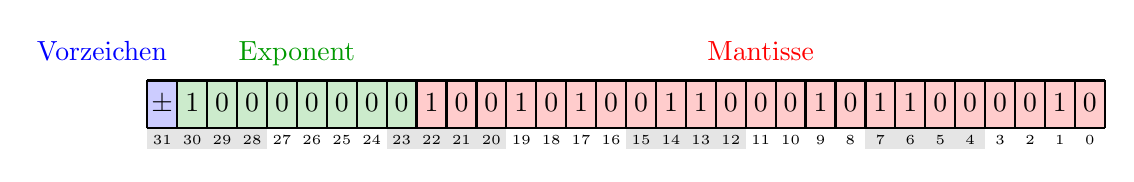
\begin{tikzpicture}[>=latex,thick,scale=0.38]

\definecolor{darkgreen}{rgb}{0,0.6,0}
\fill[color=blue!20]      (0,-0.8) rectangle (1,0.8);
\fill[color=darkgreen!20] (1,-0.8) rectangle (9,0.8);
\fill[color=red!20]       (9,-0.8) rectangle (32,0.8);

\node[color=blue]      at ( 1  ,0.8) [above left] {Vorzeichen\strut};
\node[color=darkgreen] at ( 5  ,0.8) [above] {Exponent\strut};
\node[color=red]       at (20.5,0.8) [above] {Mantisse\strut};

\fill[color=gray!20] ( 0,-0.8) rectangle ( 4,-1.5);
\fill[color=gray!20] ( 8,-0.8) rectangle (12,-1.5);
\fill[color=gray!20] (16,-0.8) rectangle (20,-1.5);
\fill[color=gray!20] (24,-0.8) rectangle (28,-1.5);

\foreach \k in {0,...,31}{
	\node at ({31.5-\k},{-1.2}) {\tiny \k};
}

\draw (0,0.8)--(32,0.8);
\foreach \x in {0,...,32}{
	\draw (\x,-0.8)--(\x,+0.8);
}
\draw (0,-0.8)--(32,-0.8);

\def\feld#1#2{
\node at ({#1+0.5},0) {$\mathstrut #2$};
}

\feld{0}{\pm}

\feld{1}{1}
\feld{2}{0}
\feld{3}{0}
\feld{4}{0}
\feld{5}{0}
\feld{6}{0}
\feld{7}{0}
\feld{8}{0}

\feld{9}{1}
\feld{10}{0}
\feld{11}{0}
\feld{12}{1}
\feld{13}{0}
\feld{14}{1}
\feld{15}{0}
\feld{16}{0}
\feld{17}{1}
\feld{18}{1}
\feld{19}{0}
\feld{20}{0}
\feld{21}{0}
\feld{22}{1}
\feld{23}{0}
\feld{24}{1}
\feld{25}{1}
\feld{26}{0}
\feld{27}{0}
\feld{28}{0}
\feld{29}{0}
\feld{30}{1}
\feld{31}{0}

\end{tikzpicture}
\end{center}
Die Ganzzahl $\texttt{10000000}_2=128_{10}$ im Exponentenfeld
muss um $127$ verringert werden um den Exponenten $1$ zu ergeben.

Die grösste und kleinste mit einem \texttt{float} darstellbare Zahl ist
somit
\begin{align*}
\texttt{1.11111111111111111111111}_2 \cdot 2^{\phantom{-}128}
&=
3.4028232_{10}\cdot 10^{\phantom{-}38}
\\
\texttt{1.00000000000000000000000}_2 \cdot 2^{-127}
&=
5.8774717_{10}\cdot 10^{-39}
\end{align*}
Den 24 binären Mantissenbits entsprechen gut 7 Dezimalstellen.

\begin{table}
\centering
\renewcommand\arraystretch{1.15}
\begin{tabular}{|l|>{$}l<{$}|>{$}l<{$}|>{$}l<{$}|}
\hline
&\texttt{float}&\texttt{double}&\texttt{long double}\\
\hline
kleinste darstellbare Zahl    &
	1.17549\cdot 10^{-38}&2.22507\cdot 10^{-308}&3.3621\cdot 10^{-4932}\\
grösste darstellbare Zahl     &
	3.40282\cdot10^{38} &1.79769\cdot10^{308} &1.18973\cdot10^{4932}\\
$\varepsilon$                 &
	1.19209\cdot 10^{-7}&2.22045\cdot 10^{-16}&1.0842\cdot 10^{-19}\\
kleinster Exponent            & -125&-1021&-16381\\
grösster Exponent             & 128&1024&16384\\
kleinste denormalisiert Zahl: &
	1.4013\cdot 10^{-45}&4.94066\cdot 10^{-324}&3.6452\cdot 10^{-4951}\\
\hline
\end{tabular}
\caption{Eigenschaften der Gleitkommatypen \texttt{float}, \texttt{double}
und \texttt{long double}.
Die Zeile $\varepsilon$ ist die Differenz zwischen 1 und der kleinsten
darstellbaren Zahl, die grösser ist als $1$.
Einzelne Exponentenwerte haben eine spezielle Bedeutung (siehe Text),
daher fallen die kleinstmöglichen Exponenten grösser aus als aufgrund
ihrer Bitlänge zu erwarten ist.
\label{buch:table:limits}}
\end{table}


\begin{table}
\centering
\begin{tabular}{|l|c|c|c|c|}
\hline
Typ&Bytes&Mantisse&Exponent&IEEE-754\\
\hline
\texttt{half},
\texttt{binary16}    &\phantom{0}2& \phantom{0}10 & \phantom{0}5     & * \\
\texttt{float},
\texttt{binary32}    &\phantom{0}4& \phantom{0}23 & \phantom{0}8     & * \\
\texttt{extended} 
                     &\phantom{0}5& \phantom{0}29 & 10               &   \\
\texttt{double},
\texttt{binary64}    &\phantom{0}8& \phantom{0}52 & 11               & * \\
\texttt{double extended},
\texttt{long double} &          10& \phantom{0}63 & 15               & * \\
\texttt{quad}
\texttt{binary128}   &          16& 112           & 15               & * \\
\texttt{binary256}   &          32& 236           & 19               & * \\
\hline
\end{tabular}
\caption{Übliche Gleitkommatypen mit Länge der Mantisse und des Exponenten.
Die meisten Compiler implementieren nur \texttt{float} und \texttt{double},
manchmal auch noch \texttt{long double}.
Die im Standard IEEE 754-2008 definierten Typen sind in der letzten Spalte
mit einen $*$ versehen.
\label{buch:table:ieee754}}
\end{table}

\subsubsection{Gebräuchliche Formate}
Der 1985 verabschiedete Standard IEEE~754 beschreibt die heute gebräuchlichen
Implementation von Gleitkommatypen abschliessend.
Damit ist gewährleistet, dass numerische Rechnungen auf verschiedenen
Prozessoren reproduzierbare Resultate geben.

Die C++-Standardbibliothek bietet im \texttt{<limits>} Header die Möglichkeit, 
Informationen über die Datentypen zu erhalten.
In Tabelle~\ref{buch:table:limits} sind die Resultate für die
gebräuchlichsten Typen zusammengestellt.
Allerdings offenbart sich hier auch ein Problem dieser Implementation
von \texttt{<limits>}.
Wie wir weiter unten sehen werden, definiert der IEEE 754 Standard
Werte für $\pm\infty$, die kleiner sind als die angegebenen
maximalen Werte.

Aktuelle Compiler unterstützen typischerweise die Gleitkomma-Typen
\texttt{float}, \texttt{double} und \texttt{long double}.
Bei Mikrokontrollern, wo Berechnungen mit der hohen Präzision
eines \texttt{double} nur schon wegen des Platzedarfs der Werte
und des Zeitbedarfs für die Operationen kaum sinnvoll sind, ist oft
nur der \texttt{float}-Typ implementiert.
Der GNU-Compiler für die 8-bit AVR-Prozessorfamilie stellt behandelt
zum Beispiel \texttt{double} genau gleich wie \texttt{float}.
Graphikkarten unterstützen oft noch einen halben Gleitkommatyp
\texttt{binary16}, dessen Genauigkeit für die Darstellung von 3D-Objekten
ausreichend ist.

\subsubsection{Rundung}
Der IEEE 754 Standard schreibt auch vor, wie Resultate gerundet werden
müssen.
\index{Rundungs-Regel}
Bei vielen Operationen entstehen Resultate, die einen längeren 
Nachkommateil haben als in das gegeben Gleitkommaformat passt,
das Resultat muss gerundet werden.
Der Standard kennt fünf verschiedene Rundungsverfahren und empfiehlt,
dass die Funktionen wie Wurzeln, Exponentialfunktionen,
trigonometrische Funktionen und viele weitere so implementiert werden 
müssen, dass das Resultat korrekt gerundet ist.
Damit ist gemeint, dass das Resultat entsteht, in dem auf das
mathematisch exakte Resultat die gewählt Rundungs-Regel angewendet
wird.

Der Standard bezweckt mit diesen, dass man sich im Rahmen der
Rundungsgenauigkeit auch auf die letzte Stelle eines Gleitkommawertes
verlassen kann.
Dies ist keinen Selbstverständlichkeit.
Gleitkomma-Implementationen von GPUs beispielsweise erfüllen diese
\index{GPU}
Bedingung oft nicht und garantieren in ihren Spezifikation manchmal
nur korrekte Resultate mit Ausnahme der letzten 1-2 bits.

\subsubsection{Die Null}
Die Gleitkomma-Darstellung definiert, dass die Mantisse ein implizites
führends \texttt{1}-bit hat. 
In diesem Format lässt sich die Null aber nicht darstellen, es ist
also eine separate Definition nötig:
\begin{itemize}
\item Vorzeichen $\texttt{0}$ oder $\texttt{1}$ erlaubt die Unterscheidung
zwischen $+0$ und $-0$.
\item Alle Exponentenbits $=\texttt{0}$.
\item Alle Mantissenbits $=\texttt{0}$.
\end{itemize}
Dies ist ein Spezialfall einer denormalisierten Zahl (siehe weiter unten)

\subsubsection{Unendlich grosse Werte}
Im Laufe einer numerischen Berechnung kann es vorkommen, dass die Resultate
so gross werden, dass nicht mehr im gegebenen Gleitkommatyp gespeichert
werden könne.
Der Standard verlangt, dass diese Situation durch einen spezielle Wert
für unendlich grosse Zahlen wiedergegeben werden kann, der wie
folgt definiert ist:
\begin{itemize}
\item Vorzeichenbit \texttt{0} oder \texttt{1} um zwischen
$+\infty$ und $-\infty$ unterscheiden zu können.
\item Alle Exponenten-Bits $= \texttt{1}$
\item Alle Mantissenbits $=\texttt{0}$
\end{itemize}
Dies bedeutet, dass der grösste nutzbare Exponent des $\texttt{float}$-Typs
nur noch $127$ ist.

\subsubsection{Denormalizierung}
\index{denormalisierte Zahl}%
Die Mantisse einer Gleitkommazahl beginnt immer mit einer 1, die aber
nicht gespeichert wird.
Wird eine Zahl kleiner als mit dem zur Verfügung stehenden Exponenten-Bereich
darstellbar, kann sie nicht mehr in diesem Format gespeichert werden.
Um solche Zahlen darzustellen, wurde vom Standard einem Exponenten aus
lauter \texttt{0} eine besondere Bedeutung gegeben.
Für den Typ \texttt{float} entspricht er nicht mehr dem Exponenten $-127$
sondern $-126$ und das implizite führend Bit der Mantisse ist jetzt 0.
Mit diesen sogenannten denormalisierten Zahlen lassen sich noch kleinere
Wert darstellen, die aber nicht mehr so präzis sind, weil sie weniger
signifikante Stellen aufweisen.

\subsubsection{Vor- und Nachteile}
\begin{itemize}
\item[$\oplus$] Konstanter relativer Fehler
\item[$\oplus$] Dank des grossen Wertebereiches sind Über- und Unterlauf
unwahrscheinlich.
\item[$\ominus$] Der kleinste Gleitkommatyp ist bereits so gross wie
der gebräuchlichste Ganzzahltyp,
Gleitkommazahlen brauchen mehr Platz.
\item[$\ominus$] Geschwindigkeit: sofern keine Hardware-Beschleunigung
zur Verfügung steht sind Gleitkomma-Operationen deutlich langsamer
als Operationen mit Festkomma-Zahlen.
\item[$\ominus$]
In einer Multi-Core CPU hat nicht unbedingt jeder Kern eine Gleitkomma-Einheit.
Gleitkommaoperationen in verschiedenen Threads können sich also gegenseitig
behindern.
\end{itemize}

%
% Hochpräzisionsbibliotheken
%
\subsection{Hochpräzisionsbibliotheken
\label{buch:subsection:mp}}
TODO: GMP

%
% effekte.tex
%
% (c) 2020 Prof Dr Andreas Müller, Hochschule Rapperswil
%
\section{Numerische Effekte
\label{buch:section:numerische-effekte}}
\rhead{Numerische Effekte}

\subsection{Auslöschnung}

\subsection{Verschmierung}


%
% iteration.tex
%
% (c) 2020 Prof Dr Andreas Müller, Hochschule Rapperswil
%
\section{Iteration
\label{buch:section:iteration}}
\rhead{Iteration}
Die meisten numerischen Problemlösungen mit einem Computer nutzen deren
Fähigkeit aus, dieselbe Rechnung immer wieder zu wiederholen, bis zum
Beispiel die gewünschte Genauigkeit erziehlt ist.
\index{Iteration}%
Es lohnt sich daher ganz unabhängig irgendwelchen Einschränkungen 
der Computer-Hardware zu überlegen, was passiert, wenn man eine
Funktion $f\colon \mathbb R\to\mathbb R$ immer wieder auf ihren eigenen
Output anwendet, wie das zum Beispiel der Code in einer Schleife
bei jedem Durchlauf macht.
\index{Hardware}%

In diesem Abschnitt ist also
\[
f\colon \mathbb{R}\to\mathbb{R} : x\mapsto f(x)
\]
eine differenzierbare Funktion.
\index{Funktion!differenzierbar}%
\index{differenzierbare Funktion}%
Mit einem gegebenen Startwert $x_0\in\mathbb R$ lässt sich durch
wiederholte Anwendung von $f$ die Folge
\[
x_0,\; x_1 = f(x_0),\; x_2 = f(x_1),\; x_3 = f(x_2),\; x_4 = f(x_3),\dots
\]
konstruieren.
\index{Iterationsfolge}%

Ist der Punkt $x^*$ ein {\em Fixpunkt} der Funktion $f(x)$, ist also
$f(x^*)=x^*$,
\index{Fixpunkt}%
dann ist die mit $x_0=x^*$ gebildete Iterationsfolge konstant.
Es stellt sich damit automatisch die Frage, was mit einem von $x^*$
abweichenden Startwert passiert.
Entfernen sich die Werte $x_k$ von $x^*$
oder konvergiert die Folge am Ende gegen $x^*$?
\index{Konvergenz}%

%
% Beispiele
%
\subsection{Beispiele}
Wir illustrieren die verschiedenen Situation, die beim Iterieren der
Funktion $f$ auftreten können an einigen Beispielen.

\begin{beispiel}
\label{section:beispiel:sqrtiteration}
Wir betrachten die Funktion 
\[
f\colon \mathbb{R}\to\mathbb{R} : x\mapsto \sqrt{x+2}
\]
Die Iterationsfolge ausgehend vom Startwert $x_0=0$ ist in
Tabelle~\ref{buch:table:sqrtiteration} dargestellt.
\index{Startwert}%

\begin{table}
\centering
\renewcommand\arraystretch{1.15}
%
% sqrtiteration.tex -- generated by sqrtiteration.m
%
% (c) 2020 Prof Dr Andreas Müller Hochschule Rapperswil
%
\begin{tabular}{|>{$}r<{$}|>{$}r<{$}|>{$}r<{$}|>{$}r<{$}|}
\hline
   k & x_k                           & \delta_k = 2-x_k     & \delta_{k-1} / \delta_{k} \\
\hline
  0 &             0.0000000000000000 &   2.0000000000000000 &        \\
  2 &             1.4142135623730951 &   0.5857864376269049 & 3.4142 \\
  3 & \underline{1.8}477590650225735 &   0.1522409349774265 & 3.8478 \\
  4 & \underline{1.9}615705608064609 &   0.0384294391935391 & 3.9616 \\
  5 & \underline{1.99}03694533443939 &   0.0096305466556061 & 3.9904 \\
  6 & \underline{1.997}5909124103448 &   0.0024090875896552 & 3.9976 \\
  7 & \underline{1.999}3976373924085 &   0.0006023626075915 & 3.9994 \\
  8 & \underline{1.9998}494036782890 &   0.0001505963217110 & 3.9998 \\
  9 & \underline{1.9999}623505652022 &   0.0000376494347978 & 4.0000 \\
 10 & \underline{1.99999}05876191524 &   0.0000094123808476 & 4.0000 \\
 11 & \underline{1.999997}6469034038 &   0.0000023530965962 & 4.0000 \\
 12 & \underline{1.999999}4117257645 &   0.0000005882742355 & 4.0000 \\
 13 & \underline{1.9999998}529314358 &   0.0000001470685642 & 4.0000 \\
 14 & \underline{1.9999999}632328584 &   0.0000000367671416 & 4.0000 \\
 15 & \underline{1.99999999}08082147 &   0.0000000091917853 & 4.0000 \\
 16 & \underline{1.999999997}7020537 &   0.0000000022979463 & 4.0000 \\
 17 & \underline{1.999999999}4255133 &   0.0000000005744867 & 4.0000 \\
 18 & \underline{1.9999999998}563782 &   0.0000000001436218 & 4.0000 \\
 19 & \underline{1.9999999999}640945 &   0.0000000000359055 & 4.0000 \\
 20 & \underline{1.99999999999}10236 &   0.0000000000089764 & 4.0000 \\
 21 & \underline{1.999999999997}7558 &   0.0000000000022442 & 3.9998 \\
 22 & \underline{1.999999999999}4389 &   0.0000000000005611 & 3.9996 \\
 23 & \underline{1.9999999999998}597 &   0.0000000000001403 & 3.9984 \\
 24 & \underline{1.9999999999999}649 &   0.0000000000000351 & 4.0000 \\
 25 & \underline{1.99999999999999}11 &   0.0000000000000089 & 3.9500 \\
 26 & \underline{1.999999999999997}8 &   0.0000000000000022 & 4.0000 \\
 27 & \underline{1.999999999999999}3 &   0.0000000000000007 & 3.3333 \\
 28 & \underline{1.9999999999999998} &   0.0000000000000002 & 3.0000 \\
 29 & \underline{2.0000000000000000} &   0.0000000000000000 &        \\
 30 & \underline{2.0000000000000000} &   0.0000000000000000 &        \\
\hline
\end{tabular}

\caption{Iterationsfolge für die Funktion $f(x)=\sqrt{x+2}$ ausgehend
vom Startwert $x_0=0$.
\label{buch:table:sqrtiteration}}
\end{table}

Die Werte konvergieren offenbar gegen den Wert $2$, 
In der dritten Spalte steht die Abweichung $\delta_k$ des $k$-ten Folgengliedes
vom Grenzwert $2$.
Mit jeder Iteration wird der Fehler um den Faktor 4 kleiner, wie die
vierte Spalte zeigt, in der Quotient aufeinanderfolgender Fehler
berechnet ist.

Dieses Verhalten des Fehlers kann man auch analytisch verstehen.
Nehmen wir an, dass $x_n = 2 + \delta_n$ und versuchen wir 
$x_{n+1}$ zu berechnen.
Indem wir die Funktion $f(x)$ im Punkt $x=2$ mit Hilfe der Ableitung
linear approximieren, erhalten wir wegen
\[
f'(x) = \frac{1}{2\sqrt{x+2}}
\]
den Wert
\[
x_{n+1} = f(x_n) = f(2 + \delta_n)
\approx
f(2) + f'(2)\cdot \delta_n
2 + \underbrace{\frac14\cdot \delta_n}_{\displaystyle\approx\delta_{n+1}}
\]
für $x_{n+1}$.
Der Fehler von $x_{n+1}$ ist also $\delta_{n+1}\approx\frac14\delta_n$.
In jedem Iterationsschritt gewinnen wir daher etwa 2 bit Genauigkeit.
Für die 52 bit Mantisse des \texttt{double} Typs brauchen wir also
etwa 26 Iterationen.
\end{beispiel}

\begin{beispiel}
\label{buch:beispiel:logistisch3}
Wir betrachten die Funktion
\[
f(x) = 3x(1-x).
\]
\index{logistische Funktion!mit $\lambda=3$}%
Sie hat zwei Fixpunkte, die man durch Lösen der quadratischen
Gleichung
\index{quadratische!Gleichung}%
\[
f(x^*)=x^*
\quad\Rightarrow\quad
x^*=-3x^{*2}+3x^*
\quad\Rightarrow\quad
3x^{*2}-2x^*=3x^*(x^*-{\textstyle\frac23})=0
\quad\Rightarrow\quad
x^*=
\begin{cases}
0      &\\
\frac23&
\end{cases}
\]
findet.

Für einen Startwert $x_0$ nahe des Fixpunktes $x^*=0$ gilt
\[
f(\delta)
=
3\delta(1-\delta)
=
3\delta - 3\delta^2.
\]
Für kleine Werte von $\delta$ kann man den quadratischen Term vernachlässigen
und sieht, dass der Fehler durch die Iteration verdreifacht wird.
Konvergenz zu diesem Fixpunkt ist also nicht möglich.

Für den Fixpunkt $x^* = \frac23$ finden wir
\begin{equation}
f({\textstyle\frac23}+\delta)
=
3({\textstyle\frac23}+\delta)({\textstyle\frac13}-\delta)
=
\frac{(2+3\delta)(1-3\delta)}3
=
\frac{2-3\delta+9\delta^2}{3}
=
\frac23 - \delta  + 9\delta^2
\label{buch:equation:logistic3error}
\end{equation}
Der Fehler $\delta$ wird zu $ -\delta(1-9\delta) $, er ändert also sein
Vorzeichen.
\index{Fehler}%
Ist $\delta>0$ wird der Fehlerbetrag wird nur um den Faktor $1-9\delta < 1$
reduziert.
Ist aber $\delta <0$, dann ist $1-9\delta>0$, der Fehlerbetrag wird wieder
vergrössert.

Sei jetzt $\delta>0$, wir wollen den Fehler nach zwei Iterationsschritten
berechnen.
Nach dem ersten ist der Fehler $\delta(1-9\delta)$, nach dem zweiten
\[
\delta(1-9\delta)(1-\delta(1-9\delta))
=
\delta(1-18\delta + 162\delta^2-729\delta^3).
\]
Für kleines $\delta$ können die Terme höhrer als erster Ordnung
vernachlässigt werden und man kann schliessen, dass der Fehler nach
zwei Iterationen tatsächlich um den Faktor $(1-18\delta)$ kleiner
geworden ist.

\begin{figure}
\centering
\includegraphics{chapters/10-arithmetik/figures/iteration.pdf}
\caption{Ein Fixpunkt $x^*$ der Funktion $f(x)$ manifestiert sich als
Schnittpunkt des Graphen $y=f(x)$ mit der $45^\circ$-Geraden.
\index{Schnittpunkt}%
\index{Graph}%
Die Iterationsfolge ausgehend von einem Startwert $x_0$ wird als
Treppenkurve zwischen dem Graphen von $f$ und der $45^\circ$-Geraden
sichtbar.
\index{Iterationsfolge}%
\label{buch:figure:iterationprinzip}}
\end{figure}

Wir möchten wissen, wieviele Iterationsschritte nötig sind, um eine
bestimmte Genauigkeit zu erreichen.
Wir möchten also den Fehler $\delta_{2n}$ vorgeben und das zugehörige
$n$ bestimmen.
Wie wir soeben berechnet haben, nimmt der Betrag des Fehlers zwischen
den Schritten $k$ und $k+2$ gemäss
\[
\delta_{k+2} = \delta_{k} (1-18\delta_k)
\]
um den Faktor $(1-18\delta_k)$ ab.
Es ist übersichtlicher, mit dem Logarithmus des Fehlers zu rechnen.
\index{Logarithmus}%
Dieser verändert sich gemäss
\[
\log \delta_{k+2}
=
\log \delta_{k} + \log(1-18\delta_k)
\approx
\log\delta_k - 18\delta_k,
\]
wobei wir für den zweiten Term die lineare Approximation aus der
Taylor-Reihe
\index{Taylor-Reihe}%
\index{lineare!Approximation}%
\index{Approximation!linear}%
\[
\log (1+x) = x - \frac{x^2}2 + \frac{x^3}3 -\dots
\]
von 
$\log x $ an der Stelle $x=1$ verwendet haben.
Zwischen $\delta_0$ und $\delta_{2n}$ bedeutet dies
\[
\log\delta_{2n}
=
\log\delta_0
-18
\sum_{k=0}^{n-1} \delta_{2k}
\qquad\Rightarrow\qquad
\frac1{18}
\log\frac{\delta_0}{\delta_{2n}}
=
\sum_{k=0}^{n-1}\delta_{2k}.
\]
Da der Fehler immer kleiner wir, kann man für eine erste grobe Abschätzung
\index{Abschätzung}%
der Summe auf der rechten Seite die grössten und kleinsten Terme
verwenden, um die Summe nach und unten und oben durch
\[
n\delta_{2n-2}
\le
\sum_{k=0}^{n-1}\delta_{2k}
\le
n\delta_0
\]
abzuschätzen.
Einsetzen ergibt
\[
n\delta_{2n-2}
\le
\frac{1}{18}
\log\frac{\delta_{0}}{\delta_{2n}}
\le
n\delta_0
\quad\Rightarrow\quad
\frac{1}{18\delta_0}
\log\frac{\delta_{0}}{\delta_{2n}}
\le
n
\le
\frac{1}{18\delta_{2n-2}}
\log\frac{\delta_{0}}{\delta_{2n}}
<
\frac{1}{18\delta_{2n}}
\log\frac{\delta_{0}}{\delta_{2n}}.
\]
Eine Verbesserung um zwei Stellen von $\delta_0=0.01$ auf $\delta_{2n}=0.0001$
braucht also zwischen $25$ und $2558$ Iterationen.
\end{beispiel}

%
% Graphische Analyse
%
\subsection{Graphische Analyse
\label{buch:section:graphischeanalyse}}
\index{graphische Analyse einer Iterationsfolge}%
\index{Iterationsfolge!graphische Konvergenzanalyse}%
Ein Fixpunkt der Funktion $f(x)$ manifestiert sich in einem 
Schnittpunkte des Graphen von $f$ mit der $45^\circ$-Geraden
$y=x$ wie in Abbildung~\ref{buch:figure:iterationprinzip}.
\index{Graph}%
\index{45grad@$45^\circ$-Gerade}%
\index{Schnittpunkt}%
Die Iterationsfolge $x_n$ kann graphisch wie folgt dargestellt
werden.
\index{Iterationsfolge}%
Ausgehend vom Wert $x_n$ auf der $x$-Achse folgt man der Vertikalen,
bis man auf den Graphen der Funktion $f$ trifft, dies liefert den
Wert $y_n=f(x_n)$.
Dieser soll jetzt als neuer $x$-Wert verwendet werden.
Dazu folgt man der Horizontalen bis zur $45^\circ$-Geraden,
die $x$-Koordinate des Schnittpunktes ist $x_{n+1}$.
So entsteht Treppenlinie in Abbildung~\ref{buch:figure:iterationprinzip}.
\index{Treppenlinie}%

%
% Konvergenzbedingung
%
\subsection{Konvergenzbedingung
\label{buch:iteration:subsection:konvergenzbedingung}}
%
% graphisch0.tex
%
% (c) 2020 Prof Dr Andreas Müller, Hochschule Rapperswil
%
\begin{figure}
\centering
\includegraphics{chapters/10-arithmetik/figures/normal.pdf}
\includegraphics{chapters/10-arithmetik/figures/negativ.pdf}
\caption{Die Fixpunktiteration $x_{n+1}=f(x_n)$ konvergiert gegen
den Fixpunkt $x^*$ falls $|f'(x^*)|<1$ mit
mindestens linearer Konvergenzgeschwindigkeit.
\label{buch:figure:fixpunkt:normal}}
\end{figure}

%
% graphisch1.tex
%
% (c) 2020 Prof Dr Andreas Müller, Hochschule Rapperswil
%
\begin{figure}
\centering
\includegraphics{chapters/10-arithmetik/figures/divergent.pdf}
\includegraphics{chapters/10-arithmetik/figures/negdiv.pdf}
\caption{Die Fixpunktiteration $x_{n+1}=f(x_n)$ mit Fixpunkt $x^*$
divergiert für $|f'(x^*)|>1$.
\label{buch:figure:fixpunkt:divergent}}
\end{figure}

Aus der graphischen Analyse von Abschnitt~\ref{buch:section:graphischeanalyse}
kann man jetzt leicht Kriterien ableiten, wann die Iterationsfolge
konvergent ist.
Die Situation in Abbildung~\ref{buch:figure:iterationprinzip}
tritt zum Beispiel immer ein, wenn in einer Umgebung von $x^*$ 
der Graph der Funktion $f$ zwischen der horizontalen und der 
$45^\circ$-Geraden verläuft, oder anders ausgedrückt, wenn
\[
\begin{aligned}
x^* &< f(x) < x &&& &\text{für $x>x^*$ und} \\
x^* &> f(x) < x &&& &\text{für $x<x^*$}
\end{aligned}
\]
gilt.

Ist dagegen der Graph von $f$ in einer Umgebung von $x^*$ steiler als
die $45^\circ$-Gerade, dann gilt 
\begin{equation}
f(x) \;\begin{cases}
> x&\qquad\text{für $ x>x^*$}\\
< x&\qquad\text{für $ x<x^*$.}
\end{cases}
\label{buch:equation:konvergenzbedingung}
\end{equation}
Es folgt dann
\[
x_{n+1} = f(x_n)
\;
\begin{cases}
> x_n&\qquad \text{für $x_n>x^*$}\\
< x_n&\qquad \text{für $x_n<x^*$.}\\
\end{cases}
\]
In beiden Fällen ist $x_{n+1}$ weiter vom Fixpunkt $x^*$ entfernt
als $x_n$, die Folge kann also nicht konvergieren.
Die beiden Situationen sind in den Abbildungen
\ref{buch:figure:fixpunkt:normal} und
\ref{buch:figure:fixpunkt:divergent}
dargestellt.

Allerdings ist die Bedignung \ref{buch:equation:konvergenzbedingung}
noch etwas zu speziell.
Der Funktionswert $f(x_n)$ darf durchaus auch kleiner als $x^*$ werden,
wenn nur der Betrag der Differenz zu $x^*$ abnimmt, wenn also gilt
\begin{equation}
|x^* - f(x_n)| < |x^*-x_n|
\label{buch:equation:konvergenzbereich}
\end{equation}
Diese Bedingung ist genügend nahe bei $x^*$ erfüllt, wenn
$|f'(x^*)| < 1$ ist.
Andererseits liegt Divergenz vor, wenn 
\[
|x^* - f(x_n)| > |x^*-x_n|,
\]
was nahe bei $x^*$ erfüllt ist, wenn $|f'(x^*)|>1$ gilt.
Wir fassen diese Resultate im folgenden Satz zusammen.

\begin{satz}
\label{buch:satz:konvergenzkriterium}
\index{Konvergenzkriterium}%
\index{Iterationsfolge!Konvergenzkriterium}%
Die Iterationsfolge $x_{n+1}=f(x_n)$ der Funktion $f(x)$ mit Fixpunkt
$x^*=f(x^*)$ konvergiert für einen Startwert $x_0$ nahe genug bei $x^*$,
wenn $|f'(x^*)|<1$, sie divergiert, wenn $|f'(x^*)|>1$.
\end{satz}

%
% Die Logistische Gleichung
%
\subsection{Die logistische Gleichung
\label{buch:subsection:logistisch}}
Die logistische Gleichung ist 
\index{logistische Gleichung}%
\[
f_\lambda(x) = \lambda x(1-x)
\]
mit dem positiven Parameter $\lambda$.
Im Beispiel auf Seite~\pageref{buch:beispiel:logistisch3} haben wir
diese Funktion bereits einmal angetroffen mit dem Parameterwert
$\lambda=3$.
Eine detailliertere Untersuchung des Konvergenzverhaltes der Iterationen
dieser Funktionen ist im Kapitel~\ref{chapter:logistic} zu finden.

Der Graph von $f_\lambda(x)$ ist eine Parabel, die die $x$-Achse
in den Punkten $(0,0)$ und $(1,0)$ schneidet.
\index{Parabel}%
Das Maximum wird bei $x=\frac12$ angenommen und ist
$f_\lambda(\frac12)=\lambda/4$.
Die Funktion bildet also das Intervall $[0,1]$ wieder in das selbe Intervall
ab, wenn $0\le \lambda\le 4$.

Wir berechnen die Fixpunkte von $f_\lambda(x)$ im Intervall $[0,1]$, also
die Lösungen der quadratischen Gleichung
\[
x^*  = \lambda x^* (1-x^*)
\quad\Rightarrow\quad
\lambda x^{*2} +(1-\lambda)x^*
=
x^* (\lambda x^* + 1-\lambda) 
=0
\quad\Rightarrow\quad
x^*
=
\begin{cases}
0&\\
\displaystyle \frac{\lambda-1}{\lambda}.&
\end{cases}
\]
Für $\lambda<1$ gibt es keinen weitere Fixpunkt im Intervall $[0,1]$, für
$\lambda>1$ ist $(\lambda-1)/\lambda<1$ immer im Intervall.

Zur Beurteilung der Konvergenz der Iterationsfolge müssen wir die Ableitung
von $f_\lambda$ im Fixpunkt berechnen.
Die Ableitung ist $f'_\lambda(x)=\lambda (1-2x)$, also gilt in den Fixpunkten
\begin{align*}
f_\lambda'(0)
&=
\lambda
\\
f_\lambda\biggl(\frac{\lambda-1}{\lambda}\biggr)
&=
\lambda\biggl( 1-2
\biggl(\frac{\lambda-1}{\lambda}\biggr)\biggr)
=
\lambda-2(\lambda-1)
=
2-\lambda.
\end{align*}
Daraus liest man mit dem Konvergenzkriterium von
Satz~\ref{buch:satz:konvergenzkriterium} ab, dass Konvergenz zum Punkte
$(\lambda-1)/\lambda$ vorliegt für $\lambda \in (1,3)$.
\index{Konvergenzkriterium}%
Für $\lambda>3$ divergiert die Iterationsfolge.

Im Beispiel auf Seite~\pageref{buch:beispiel:logistisch3} haben wir
wir den Grenzfall $\lambda=3$ untersucht und festgestellt, dass die
Iterationsfolge gerade noch konvergiert, allerdings sehr langsam.
Man beachte, dass das Kriterium \eqref{buch:equation:konvergenzbereich}
in diesem Fall nicht erfüllt ist.
Für $\lambda<1$ konvergiert die Iterationsfolge zum Nullpunkt.

Wie verhält sich die Folge im Grenzfall $\lambda=1$?
Auch in diesem Grenzfall ist das Kriterium nicht erfüllt, wir müssen
das Problem als wieder gesondert analysieren.
Es gilt
\[
x_{n+1} = x_n(1-x_n) = x_n-x_n^2.
\]
Für $x_n>0$ folgt also, dass $0<x_{n+1} < x_n$ ist, die Folge wird also
konvergieren.
Allerdings ist die Konvergenz wieder ähnlich langsam wie im Falle
$\lambda=3$.
Für einen Wert $x_n<0$ ist allerdings $x_{n+1} = x_n - x_n^2 < x_n$,
d.~h.~die Folge divergiert.
Dieses Verhalten lässt sich auch allgemein formulieren.

\begin{satz}
\label{buch:satz:kritischekonvergenz}
Falls $f'(x^*)=1$, dann konvergiert die Iterationsfolge für einen
Startwert $x_0$ genügend nahe und grösser als $x^*$ wenn $f''(x^*)<0$ 
und sie divergiert für $f''(x^*)>0$.
Für einen Startwert genügend nahe und kleiner als $x^*$ dagegen
konvergiert die Iterationsfolge für $f''(x^*)<0$ und divergiert für
$f''(x^*)>0$.
\end{satz}

\begin{proof}[Beweis]
Wir entwickeln die Funktion $f$ im Punkt $x^*$ die Potenzreihe
\index{Potenzreihe}%
\begin{align*}
f(x^*+\delta)
&=
f(x^*) + f'(x^*)\cdot\delta + \frac12f''(x^*)\cdot \delta^* + O(\delta^3)
\\
&=
x^* + \delta + \frac12f''(x^*)\delta^2
\end{align*}
Die Entfernung zu Fixpunkt ist
\[
|f(x^*+\delta)-x^*|
\approx
|\delta  + \frac12f''(x^*)\delta^2|
=
|\delta|\cdot |1 + \frac12f''(x^*)\delta|.
\]
Ob die Entfernung wird genau dann grösser, wenn $f''(x^*)\delta$ positiv ist.
sie wird kleiner, wenn $f''(x^*)\delta$ negativ sind.
Der erste Fall tritt ein, wenn $\delta$ und $f''(x^*)$ gleiches
Vorzeichen haben.
Für Werte grösser als $x^*$ heisst das, dass $f''(x^*)>0$ sein muss.
Analog folgen alle anderen Fälle.
\end{proof}

Für den Fall $\lambda=3$ der logistischen Gleichung können wir den
folgenden Satz formulieren:

\begin{satz}
Falls $f'(x^*)=-1$, dann konvergiert die Iterationsfolge für einen
Startwert genügend nahe bei $x^*$, wenn $f''(x^*) <0$, sie divergiert,
wenn $f''(x^*)>0$.
\end{satz}

\begin{proof}[Beweis]
Wir verwenden wieder die Entwicklung
\begin{align*}
f(x_n)
&=
f(x^* +\delta_n)
=
f(x^*) + f'(x^*) \cdot \delta_n + \frac12 f''(x^*)\cdot \delta_n^2
+ \dots
=
x^* - \delta_n + \frac12f''(x^*)\delta_n^2 +\dots
\\
\delta_{n+1}
&=
-\delta + \frac12f''(x^*)\delta^2 \dots
\end{align*}
Daraus kann man zunächst ableiten, dass der Fehler bei jedem 
Iterationsschritt das Vorzeichen wechselt.
Wir berechnen den Fehler nach zwei solchen Schritten.
\begin{align*}
\delta_{n+2}
&=
-\delta_{n+1} + \frac12f''(x^*) \delta_{n+1}^2
=
\delta_n - \frac12f''(x^*) \delta_n^2
+
\frac12 f''(x^*) \bigl(-\delta_n + f''(x^*)\delta_n^2\bigr)^2
\\
&=
\delta_n 
-\frac12 f''(x^*)
\delta_n^2
+\frac12 f''(x^*)
\bigl( \delta_n^2 + 2f''(x^*)\delta_n^3 + f''(x^*)^2\delta_n^4\bigr)
\\
&=
\delta_n
+
f''(x^*)^2\delta_n^3
+
\frac12f''(x^*)^3\delta_n^4
+\dots
\\
&=
\delta_n (1 + f''(x^*)\delta_n^2)
\end{align*}
Die Terme höherer Ordnung als $3$ können für kleines $\delta_n$ 
vernachlässigt werden.
Nach zwei Iterationsschritten hat also der Fehler wieder das gleiche
Vorzeichen, aber der Betrag hat sich im den Faktor
\[
1+f''(x^*)\delta_n^2
\]
verändert.
Dieser Faktor ist genau dann $<1$, wenn $f''(x^*)<0$ ist.
\end{proof}

Ähnlich wie im Beispiel auf 
Seite~\pageref{buch:beispiel:logistisch3} kann man auch in diesem
Fall zeigen, dass die Konvergenz der Folge sehr langsam ist.

%
% Dritte Ableitung im Fixpunkt
%
\subsection{Dritte Ableitung im Fixpunkt
\label{buch:subsection:dritteableitungfixpunkt}}
\index{fstrich@$f'''(x)$}%
\index{dritte Ableitung}%
\index{Ableitung!dritte}%
Die bisher zusammengetragenen Sätze decken die Fälle $|f'(x^*)|=1$ mit
nicht verschwindender zweiter Ableitung $f''(x^*)\ne 0$ ab.
In einigen Fällen ist Konvergenz nicht gesichert, doch wenn Konvergenz
vorliegt, dann ist sie sehr langsam.
Speziell an dieser Situation ist, dass
$f(x)-(x^* + f'(x^*)(x-x^*))$
das Vorzeichen in einer Umgebung von $x^*$ nicht wechselt.

Noch nicht untersucht wurde der Fall $f''(x^*)=0$.
Es ist klar, dass die Konvergenzgeschwindigkeit nicht schneller
werden kann.
\index{Konvergenzgeschwindigkeit}%
Für $f'''(x^*)\ne $ folgt zudem, dass in diesem Fall
$f(x)-(x^* + f'(x^*)(x-x^*))$
das Vorzeichen in einer Umgebung von $x^*$ wechselt.
Da aber das Iterationsverfahren sehr empfindlich darauf regiert, ob
der Graph von $f$ oberhalb oder unterhalb der Geraden $y=\pm x$ 
liegt, erwarten wir ein anderes Verhalten als im Fall $f''(x^*)\ne 0$.
%
% kubisch.tex
%
% (c) 2020 Prof Dr Andreas Müller, Hochschule Rapperswil
%
\begin{figure}
\centering
\includegraphics{chapters/10-arithmetik/figures/m1kp.pdf}
\includegraphics{chapters/10-arithmetik/figures/m1kn.pdf}
\caption{Die Fixpunktiteration $x_{n+1}=f(x_n)$ mit Fixpunkt $x^*$
mit $f'(x^*)=1$ und $f''(x^*)=0$ divergiert für $f'''(x^*)>0$
und konvergiert sehr langsam für $f'''(x^*)<0$.
\label{buch:figure:fixpunkt:abl1kub}}
\end{figure}
%
\begin{figure}
\centering
\includegraphics{chapters/10-arithmetik/figures/mnkp.pdf}
\includegraphics{chapters/10-arithmetik/figures/mnkn.pdf}
\caption{Die Fixpunktiteration $x_{n+1}=f(x_n)$ mit Fixpunkt $x^*$
mit $f'(x^*)=-1$ und $f''(x^*)=0$ konvergiert sehr langsam für $f'''(x^*)>0$
und divergiert für $f'''(x^*)<0$.
\label{buch:figure:fixpunkt:ablm1kub}}
\end{figure}
%
Alle möglichen Situationen sind in den
Abbildungen~\ref{buch:figure:fixpunkt:abl1kub} und
\ref{buch:figure:fixpunkt:ablm1kub} dargestellt.

Wir gehen also davon aus, dass sich $f$ in einer Umgebung von $x^*$
in der Form
\[
f(x^*+\delta)
\approx
\tilde{f}(x^*+\delta)
=
x^* + f'(x^*)\delta + \frac1{6}f'''(x^*) \delta^3
=
x^* + s\delta + a\delta^3
\]
entwickeln lässt, wobei $s=\pm 1$ und $a\ne 0$ ist.

Der Iterationsfehler $\delta_{n+1}$ verhält sich wie
\begin{align*}
x^* + \delta_{n+1}
&=
f(x_n)
=
f(x^* + \delta_n)
=
x^* + s\delta_n + a\delta_n^3 + O(\delta_n^4).
\\
\delta_{n+1}
&=
s\delta_n + a\delta_n^3 + O(\delta_n^4)
=
\delta_n(s+a\delta_n^2) + O(\delta_n^4)
=
s\delta_n\biggl(1+\frac{a}{s}\delta_n^2\biggr) + O(\delta_n^4)
\end{align*}
Da $\delta_n^2>0$ ist, ist der Klammerausdruck genügend nahe bei $x^*$
immer positiv.
Der Betrag des Fehlers verhält sich dann wie
\[
|\delta_{n+1}|
=
|\delta_n| \cdot \biggl(1 + \frac{a}{s}\delta_n^2\biggr) + O(\delta_n^4).
\]
Ob der Fehler bei der Iteration grösser oder kleiner wird, hängt also
einzig vom Vorzeichen von $a/s$ ab.
Ist $a/s > 0$, wird der Fehler grösser, die Iterationsfolge ist divergent,
ist $a/s < 0$, wird der Fehler kleiner, die Iterationsfolge konvergiert.
Wir fassen diese Resultate zusammen im folgenden Satz.

\begin{satz}
Falls $f\colon\mathbb R\to\mathbb R$ den Fixpunkt $x^*\in\mathbb R$ hat,
und $f'(x^*)=\pm1$, $f''(x^*)=0$ und $f'''(x^*)\ne 0$ ist, dann ist die
Iterationsfolge $x_{n+1}=f(x_n)$ konvergent, falls $f'(x^*)\cdot f'''(x^*)<0$
ist, gleichbedeutend damit, wenn $f'(x^*)$ und $f'''(x^*)$ verschiedene
Vorzeichen haben.
Wenn $f'(x^*)$ und $f'''(x^*)$ das gleiche Vorzeichen haben, dann ist
die Fixpunktiterationsfolge divergent.
\end{satz}

Abbildung~\ref{buch:figure:fixpunkt:abl1kub} zeigt die Situation $f'(x^*)=1$
während Abbildung~\ref{buch:figure:fixpunkt:ablm1kub} die Situation
$f'(x^*)=-1$ abdeckt.


%
% beschleunigung.tex
%
% (c) 2020 Prof Dr Andreas Müller, Hochschule Rapperswil
%
\section{Konvergenzbeschleunigung
\label{buch:section:beschleunigung}}
\rhead{Konvergenzbeschleunigung}
Sind die Fehler einer iterativen numerischen Berechnungsmethoden
bekannt, kann die Gesetzmässigkeit der Fehler ausgenutzt werden,
sie weitgehend zu eliminieren, und so die Konvergenz des Verfahrens
zu beschleunigen.
In diesem Abschnitt wollen wir das Prinzip veranschaulichen, es
soll später bei der Berechnung von Integralen systematisch
angewendet werden.




%
% instabilitaet.tex
%
% (c) 2020 Prof Dr Andreas Müller, Hochschule Rapperswil
%
\section{Numerische Instabilität
\label{buch:section:instabilitaet}}
\rhead{Numerische Instabilitöt}








%
% kondition.tex
%
% (c) 2020 Prof Dr Andreas Müller, Hochschule Rapperswil
%
\begin{frame}
\frametitle{Konditionszahl}
\vspace{-15pt}
\begin{columns}[t]
\begin{column}{0.48\hsize}
\begin{block}{Norm einer Matrix}
\[
\|A\| = \max_{|x|\le 1} |Ax|
\]
``maximaler Streckungsfaktor''
\end{block}
\uncover<2->{%
\begin{block}{Konditionszahl}
\[
\kappa(A) = \|A\|\cdot\|A^{-1}\|
\]
\begin{itemize}
\item<3-> $\kappa(A)\simeq 1$: gut
\item<4-> $\kappa(A)$ gross: schlecht
\end{itemize}
\end{block}}
\end{column}
\begin{column}{0.48\hsize}
\uncover<5->{%
\begin{block}{Singulärwertzerlegung}
Für die Singulärwertzerlegung
\[
A=U\,\operatorname{diag}(s_1,\dots,s_n)\,V^t
\]
\uncover<7->{gilt}%
\begin{align*}
\uncover<8->{\|A\|}
&\uncover<8->{= \max_{1\le i\le n} |s_i|}
\\
\uncover<9->{\kappa(A)}
&\uncover<9->{=
\max_{1\le i\le n} |s_i| / \min_{1\le i\le n} |s_i|}
\\
&\uncover<10->{=
\max_{i,k} \frac{|s_i|}{|s_k|}}
\end{align*}
\uncover<6->{Schlechte Kondition: ``fast singulär''}
\end{block}}
\end{column}
\end{columns}
\end{frame}


\section*{Übungsaufgaben}
\aufgabetoplevel{chapters/10-arithmetik/uebungsaufgaben/}
\begin{uebungsaufgaben}
\uebungsaufgabe{1001}
\uebungsaufgabe{1002}
\end{uebungsaufgaben}






